\section{Design}

Review and evaluation of Ohmage reference application and open mHealth schema.
Review case studies. 
Design and prototype alternative trust / security approach to current OAuth2-based mechanism. 
Design new repository. 
Provide NDN-CCL and NFD support for Android. 
Trying replacing REST backend in Ohmage with NDN.

\paragraph{Challenges}

For this application in particular, NDN provides much more relevant functionality at the network layer than IP.  
So solutions in NDN have much more direct impact on the scalability, security, and ease of development; we need not build up additional layers on IP to get near the app challenges.

Cite hourglass figure 

\begin{itemize}
\item Namespace / schema design
\item Repository / storage design
\item Service composability
\item Authentication / identity assurance
\item Data provenance
\item Access auditing
\item Mobile publishing
\item Legal requirements for success
\end{itemize}


\paragraph{Approach}
Follow up on mHealth design approach from Estrin \& Sim, 2010.

\begin{itemize}
\item \textbf{Interoperable, Internet-inspired data exchange} as the backbone of the application ecosystem
\item \textbf{Thin waist of open data interchange standards} that will enable an ecosystem of sensing, storage, analysis, and user interface components to support medical discovery and evidence-based care 
\item Market-supported, patient-centered landscape of innovative health applications
\item \textbf{Patient-controlled, privacy-aware data exchange} across device, component, and application boundaries
\end{itemize}

\paragraph{mHealth Reality Check}

%% From 
%% PLOS Medicine Editors. "A reality checkpoint for mobile health: three challenges to overcome." PLoS Medicine 10.2 (2013).
%% TODO: Add to cites

\begin{itemize}
\item \textbf{Are your systems interoperable?}
Estrin \& Sim in Science, 2010.  Open mHealth. 
\item \textbf{Are you using open standards?}
WHO, 2013.  eHealth unit. 
\item \textbf{How will you evaluate?}
Greenhalgh et al. in BMC Med Res. Methodology, 2011.
Realist and meta-narrative evidence synthesis.
\end{itemize}

\subsection{Reference Application: Ohmage} 

Plan to create/port a mobile client for the Ohmage reference platform, which currently incorporates:
Mobile application, LAMP stack back-end, REST communication

Key pain point is OAuth 2.0:  Implementation relies on this � doesn�t scale to the DPU model and has numerous problems.  Quickly identified by 

Open mHealth lead architect as a primary challenge.   

Same approach (apparently) used in Human API mentioned earlier. 


\subsection{User Interface}
Begin with this, because consumer-facing. 

\subsubsection{Mobile}
\subsubsection{Website}
Start with Ohmage front end (see previous slides).
Web-based front end using NDN-JS to access derived data without location information.
Examples: http://quantifiedself.com/fitbit/ 



\subsection{NDNEx Application architecture}

Translate existing REST-based approach?  How quickly to move to a new model of data exchange where transactions are mostly about (for example) keys. 

Based on 
PEIR, the personal environmental impact report, as a platform for participatory sensing systems research. Mun, M., Reddy, S., Shilton, K., Yau, N., Burke, J., Estrin, D., ... \& Boda, P. (2009, June). Proc. ACM Mobisys 2009. 

  
Capture (Anyang / Tsinghua / UCLA) 
Storage (Tsinghua / UCLA)
Processing (Basel)
Presentation (REMAP)
Security (Michigan)


\subsubsection{Mobile application}

Design for Android. Port NFD, tools.

We are going to use the Ohmage Android client (including the Mobility module) with only the in-app storage and communication changed to NDN. 
See (Tangmunarunkit, H., et al., 2014) and also the papers on the Ohmage website. 

Note that Mobility generates activity classified data that may not require the Activity Classification DPU in the initial version.

Instance of TCP/IP Ohmage (client and server) is now up and running thanks to Haitao in Lixia�s group at UCLA.  

Initial analysis of Ohmage mobile client communication completed by Prof. Euihyun Jung�s group from Anyang Univ.   

From Basel: Today, we had an internal presentation from the Psychology Dept which explained their use of the Ohmage system that is running in Basel. Although NDNex comes too late for being applied in ongoing projects, these projects are a good source of insights about user requirements for our future NDNex system, especially the aspect of data sovereignty.


\subsubsection{Data Storage}

Approach:  One or more new NDN repo designs supporting a hierarchy of storage needs: mobile device, user private repository, temporary processing storage.

Requirements: From Open mHealth Data Storage Unit (DSU) Design and overall application architecture.

Storage at:
\begin{itemize}
\item The mobile device itself.
\item A personal data repository (which may be distributed).
\item Temporary storage for processing and visualization components. 
\end{itemize}

Current plan:  implement in Java using jNDN, for Android support. 

Design led by Jianxun in Dan Pei�s group at Tsinghua. 

\subsubsection{Processing}

Goal here is to have a few representative components implemented using NFN-style approach, not exactly the processing blocks listed above, necessarily.  

Ideally, provide composable data flow inspired by Google Cloud Dataflow, Apache Spark, etc.  

Start with GeoFencing, as activity classification is currently handled in the Mobility portion of Ohmage.  But, could also consider other application-specific processing ideas. 

\subsubsection{Visualization}
Start with Ohmage web front end
And Lifestreams?
NDN-JS and D3
Web-based front end using NDN-JS with access to geofenced location information, providing (for example) running trail visualization.
Perhaps use many GPX format visualizers.  E.g., \url{http://flowingdata.com/2014/02/05/where-people-run/}
  
\subsubsection{Location-based Content Emitter}
Web-based front end using NDN-JS with access to geofenced location information, providing location-specific content back to the mobile user.

Related to vehicular networking work. 
  
  
\subsubsection{Identity Manager}
  
  
\subsection{Trust and security}

Replacing Oauth2 for distributed processing is critical
One
entity (here, the `` user") maintains multiple publishers whose data are
consumed by many services with varying levels of access based on the: type
of data (as expressed in the name), level of granularity, and date/time
when the data was produced. ABE seems a good fit here, is it viable for
practical experimentation or do we need a directory-of-symmetric-keys or
some other approach?  If not ABE, where should we begin for our approach?
Are there existing best practices?


\subsubsection{Trust model} 
Leverage PKI as deployed
Would like to start from the same tools being used for user/gateway trust management in NDN testbed for this application.  
How to take advantage of the NDN signing infrastructure?
Certificates and delegation of authority.

\subsubsection{Identity}
Each processing block in this diagram may come from a different service provider. 
User may have different identity per service (or at least per flow). 
Each step tends to generate derived data that must also be stored and may not be associated with the original identity.  

We are exploring the idea of an ``identity manager", an application
manages the certificates (identities) that an individual uses to interact
with the various services involved in this application. Are there good
examples of \emph{user interfaces} for identity management already?  In fact,
pointers to state-of-the-art in end-user interfaces for security decision
making would be helpful. Alex doesn't think there are many. 

\subsubsection{Integrity} 

\subsubsection{Confidentiality}

Principal of minimum information. 

Access control in "data flow" model for communication between processing components, replacing Oauth (with Tsinghua and UCLA).  Extensions to support epidemiological studies incorporating semi-anonymized opt-in data across large populations. 

We will need to come up with an approach for name encryption for
this environment, in a way that still enables applications to operate on
the namespace--perhaps without having to be concerned with
decryption--once it has been decrypted and/or de-encapsulated.


\subsubsection{Data flow model support}
We imagine a data flow like model for this system:
[Publisher]->[Processing]->[Processing]->[Visualization], with each []
block being owned by a different entity and an objective to leak the
minimum amount of context to the processing components.  I'm not sure we
understand how to handle authentication /  access control of the
intermediate processing blocks, to each other and to the source/sink of
the data.  Where can we look for best practices for security in current
data flow architectures?



\subsection{Naming}

\subsubsection{Data}
Personal health data (and metadata) namespace and repository design � focusing on support for physical activity data in the first round.  
What schema? Initially, try direct mapping of Open mHealth schema to names


\textbf{Basis of design}: Open mHealth Physical Activity data schema\footnote{\url{http://www.openmhealth.org/developers/schemas/#physical-activity} and \url{http://bioportal.bioontology.org/ontologies/SNOMEDCT?p=classes&conceptid=68130003}}, as well as other schemas from Open mHealth as needed. 

\begin{listing}
\begin{minted}[frame=single,
               framesep=3mm,
               linenos=false,
               fontsize=\footnotesize,
               tabsize=2]{js}
{     
    "$schema": "http://json-schema.org/draft-04/schema#",

    "description": "This schema represents a single episode of physical activity.",
    "type": "object",
    "references": [
        {
            "description": "The SNOMED code represents Physical activity (observable entity)",
            "url": "http://purl.bioontology.org/ontology/SNOMEDCT/68130003"
        }
    ],
    "definitions": {
        "activity_name": {
            "$ref": "activity-name-1.0.json"
        },
        "length_unit_value": {
            "$ref": "../generic/length-unit-value-1.0.json"
        },
        "time_frame": {
            "$ref": "../generic/time-frame-1.0.json"
        }
    },

    "properties": {
        "activity_name": {
            "$ref": "#/definitions/activity_name"
        },
        "effective_time_frame": {
            "$ref": "#/definitions/time_frame"
        },
        "distance": {
            "description": "The distance covered, if applicable.",
            "$ref": "#/definitions/length_unit_value"
        },
        "reported_activity_intensity": {
            "description": "Self-reported intensity of the activity performed.",
            "type": "string",
            "enum": ["light", "moderate", "vigorous"]
        }
    },

    "required": ["activity_name"]
}
\end{minted}
\caption{Open mHealth Physical Activity Schema, retrieved December 28, 2014. See appendix for subschema.} 
\label{listing:physical-activity-json}
\end{listing}




How to separate this into namespace and data?
Figure~\ref{fig:ndnex-namespace}

JSON payload. 

\begin{figure}
\begin{center}
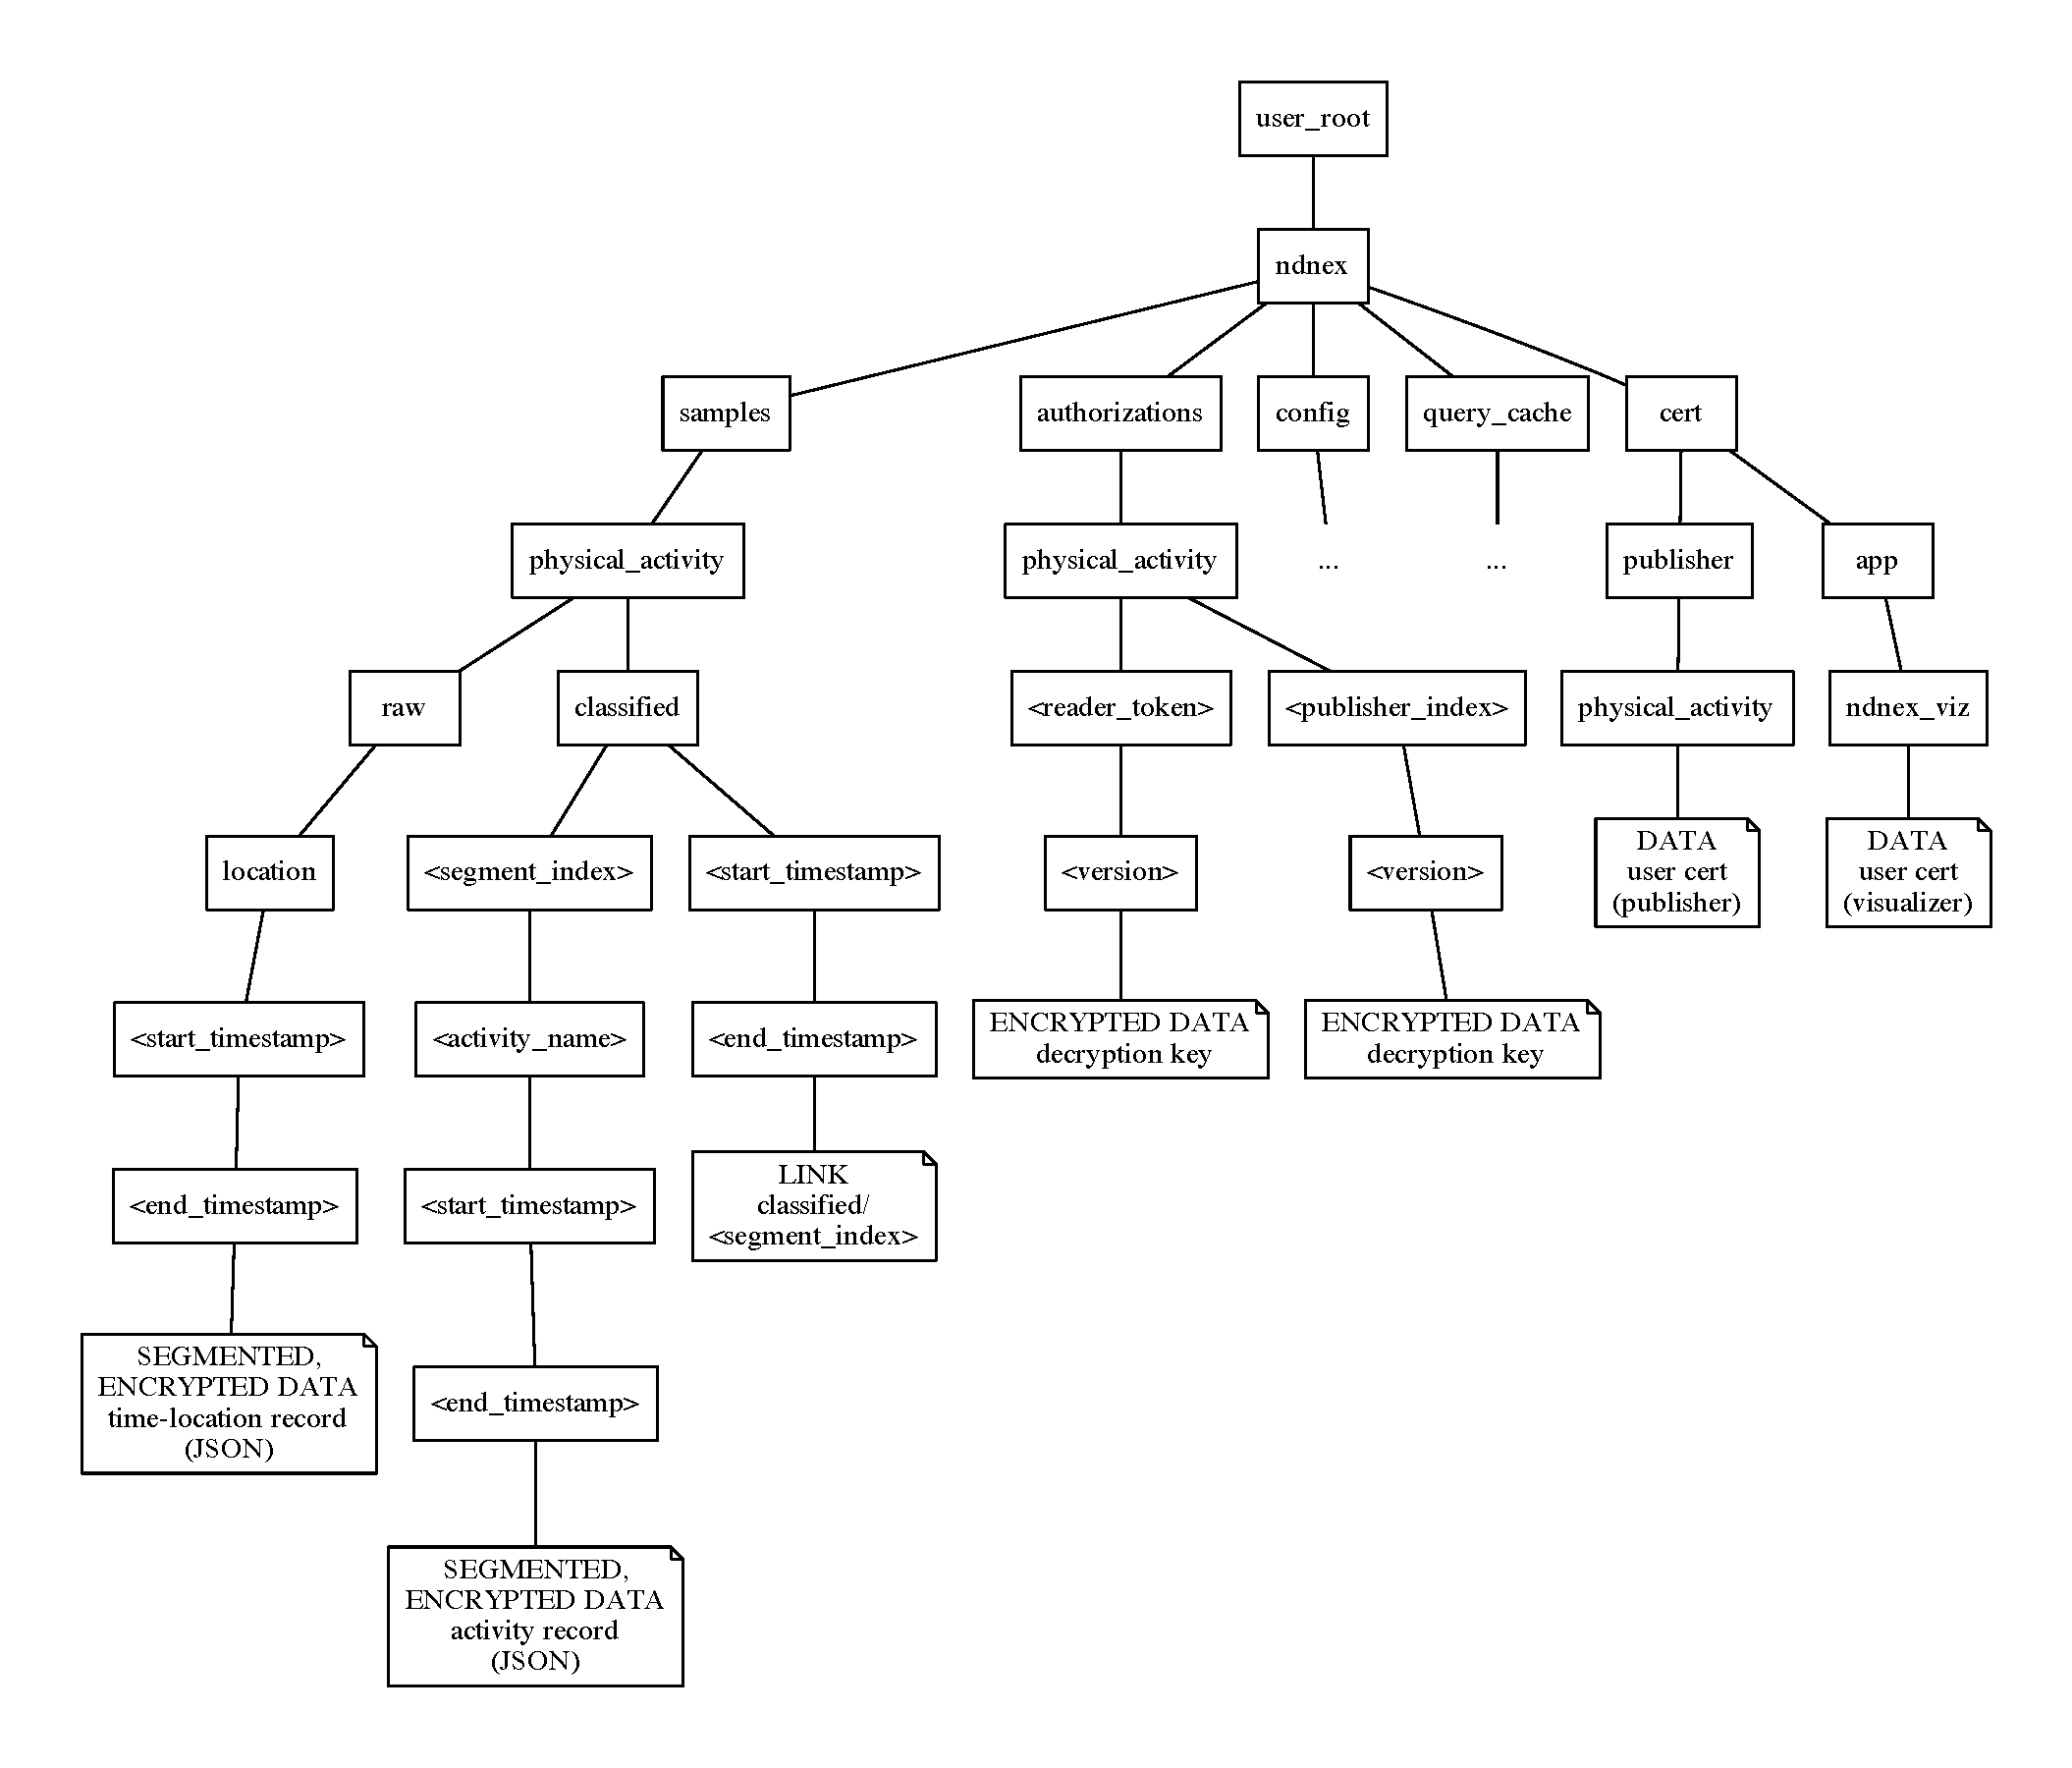
\includegraphics[width=1\textwidth]{figures/ndnex-name-top-01}
\caption{NDNEx Namespace, version 1.}
\label{fig:ndnex-namespace}
\end{center}
\end{figure}

\subsubsection{Certificates}

\subsubsection{Processing}
Borrow ideas from Named Function Networking concept for distributed processing


\subsection{Storage}

A distributed network of repos replaces the ecosystem of DSUs envisioned in the Open mHealth TCP/IP architecture. 

(Hierarchical network of repositories, similar to BAS/BMS, including both personal repositories, service provider backups for personal data, and aggregated "anonymized" stores). 

Write access control

A mechanism for delegating authority to publish into a repository is
necessary. 
\subsection{Routing \& Forwarding}
Mobile publishing support



\begin{figure}
\centering
\subfigure[Mobile publisher connected to ``home'' hub, which directly routes its publishing prefix.]{
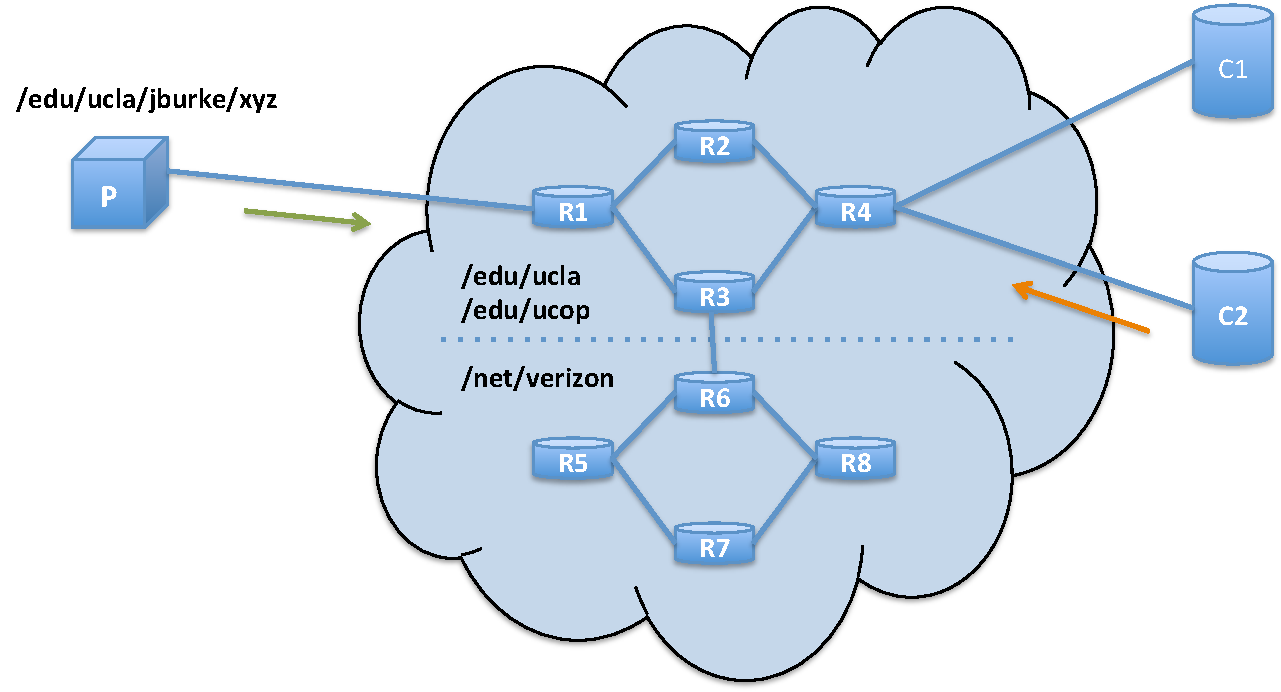
\includegraphics[width=0.45\columnwidth, keepaspectratio=true]{figures/publisher-mobility-a}
}
\subfigure[Mobile publisher connected to another hub, which does not directly route its prefix.]{
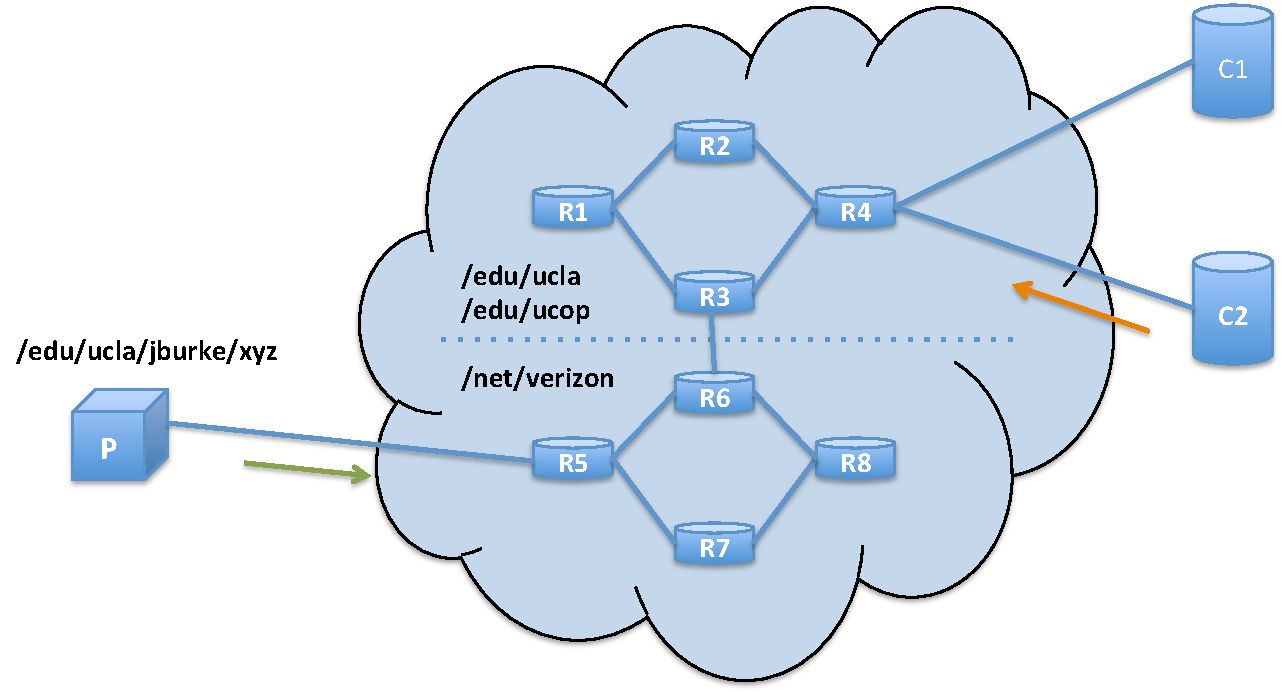
\includegraphics[width=0.45\columnwidth, keepaspectratio=true]{figures/publisher-mobility-b}
}
\caption{Mobile publisher scenario.}
\label{fig:mobilepublisher}
\end{figure}

\subsection{Distributed Processing}
Incorporate Haitao's design?
Named Function Networking style support for distributed processing with University of Basel. 

